


\chapter{Multi-structures}\label{chap:multi-structures}

\section{Introduction}

This chapter will introduce the structures that will serve as the basis for all of the concepts that will be discussed by this book. 

A \textbf{multi-structure} is a collection of points (a multi-point), a collection of paths (a multi-path), a collection of surfaces (a multi-surface), or a collection of volumes (a multi-volume). The ``type" of a multi-structure is the status of being a multi-point, a multi-path, a multi-surface, or a multi-volume. All of these structures will be assumed to exist in {\bf 3D space}.


\section{Multi-points}

~

\begin{tabular}{cc}
\parbox{0.5\textwidth}{
A \textbf{multi-point} is a superposition of points. One such superposition is depicted on the right.
} & \parbox{0.5\textwidth}{
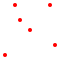
\includegraphics[scale = 0.75]{Multi-structures/Multipoints/multi-point_simple}
}
\end{tabular}

\vspace{5mm}

\begin{tabular}{cc}
\parbox{0.5\textwidth}{
When two points have the same position, the result is a point with a weight of \(2\). When three points have the same position, the result is a point with a weight of \(3\). Every point in a multi-point has associated with it a ``weight" which is the number of how many points have been stacked into the same position. The weight can be a fraction, so there can be fractional copies of a point. The weight can also be negative, so there can be ``anti-points". If the weight is \(0\), then the point is simply not included. On the right is a multi-point, where the points have different weights.
} & \parbox{0.5\textwidth}{
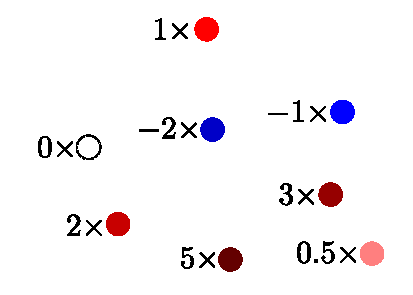
\includegraphics[scale = 0.75]{Multi-structures/Multipoints/multi-point_multiplicity}
}
\end{tabular}

\vspace{2mm}

A multi-point \(\rho\) is effectively a set of point (\(P\)) / weight (\(w\)) pairs. An arbitrary multi-point will be denoted via the notation
\[\rho = w_1 P_1 + w_2 P_2 + ... + w_N P_N\]
where \(w_i\) is the weight that is assigned to point \(P_i\). This notation effectively denotes that a multi-point is a collection/sum of points.

Each weight \(w_i\) will be assumed to be nonzero, as a point with a weight of 0 is not included as part of the multi-point. Moreover, the points will be assumed to all be unique. If a point appears multiple times, then these appearances can be condensed into a single appearance whose weight is the sum of all weights from the multiple appearances. 

Two multi-points are equivalent if and only if the collections of constituent points are equivalent with identical weights. 




\section{Multi-paths}

A path is 1D trail. An oriented path is a path that has a preferred direction as is depicted in the four examples below:
\begin{center}
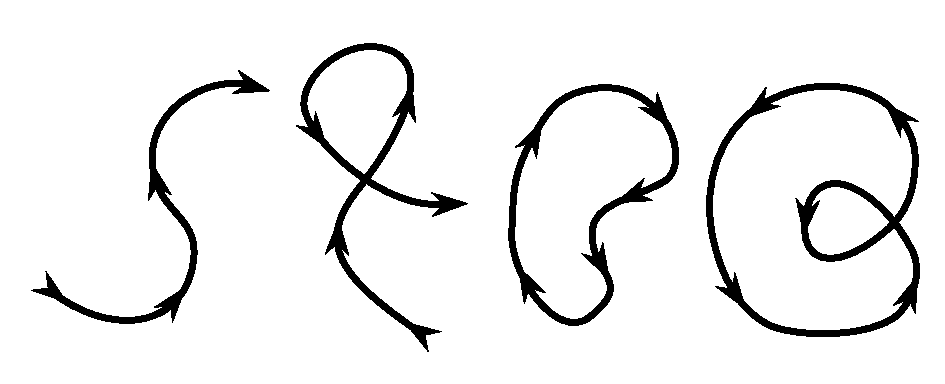
\includegraphics[scale = 0.5]{Multi-structures/Multipaths/oriented_paths}
\end{center}

\begin{tabular}{cc}
\parbox{0.5\textwidth}{
A \textbf{multi-path} is a superposition of oriented paths. One such superposition is depicted on the right.
} & \parbox{0.5\textwidth}{
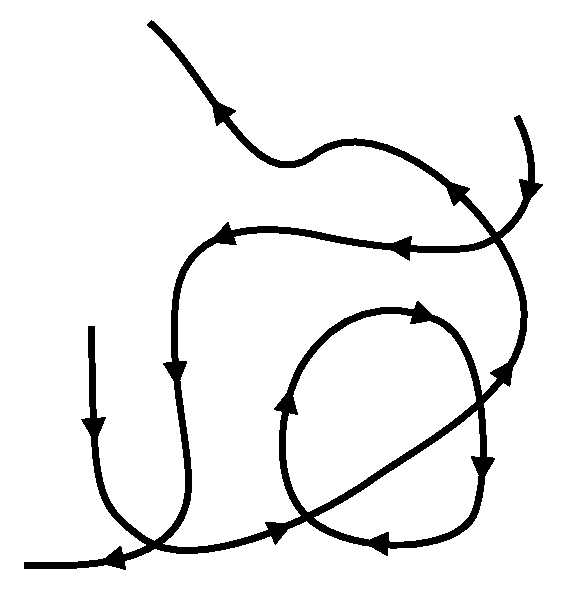
\includegraphics[scale = 0.7]{Multi-structures/Multipaths/multi-path_simple}
}
\end{tabular}

\begin{tabular}{cc}
\parbox{0.5\textwidth}{
When two oriented paths in the same multi-path are equivalent, the result is the common oriented path with a weight of \(2\). When three oriented paths in the same multi-path are the equivalent, the result is the common oriented path with a weight of \(3\). Every oriented path in a multi-path has associated with it a ``weight" which is the number of ``stacked" oriented paths. The weight can be a fraction, so there can be fractional copies of a path. {\bf If the weight is negative, then the orientation of the path is reversed and the sign is flipped to positive.} On the right is a multi-path where the paths have different weights. Note how there are no negative weights, as a negative weight merely flips the orientation of the path.  
} & \parbox{0.5\textwidth}{
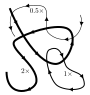
\includegraphics[scale = 0.75]{Multi-structures/Multipaths/multi-path_multiplicity}
}
\end{tabular}

A multi-path \(\mathbf{J}\) is effectively a set of oriented path (\(C\)) / weight (\(w\)) pairs:
\[\mathbf{J} = w_1 C_1 + w_2 C_2 + ... + w_N C_N\]
where \(w_i\) is the weight that is assigned to path \(C_i\). This notation effectively denotes that a multi-path is a collection/sum of oriented paths.

Each weight \(w_i\) will be assumed to be strictly positive, as an oriented path with a weight of 0 is not included as part of the multi-path, and a negative weight can be made positive while reversing the path's orientation. Moreover, the oriented paths will be assumed to all be unique. If a path appears multiple times, then these appearances can be condensed into a single appearance whose weight is the sum of all weights from the multiple appearances. If an oriented path and its reversed orientation appears, then these instances cancel out. The orientation with the smaller weight is eliminated, while the orientation with the larger weight has its weight reduced by the smaller weight. If the weights of both orientations are equal, then the orientations completely cancel each other out. It should also be noted that curves can partially cancel each other out (as illustrated below on the right). 

Two multi-paths are equivalent if and only if the networks of oriented paths are equivalent, regardless of how the network is broken up into individual oriented paths, as illustrated below. In the example on the right, the segments that are on top of each other and have opposite orientations have canceled each other out.    
\begin{center}
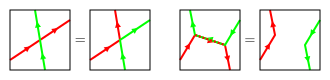
\includegraphics[scale = 0.5]{Multi-structures/Multipaths/multi-path_decomposition}
\end{center}

\begin{center}
\begin{tabular}{cc}
\parbox{0.5\textwidth}{
Unless otherwise specified, no path will be allowed to diverge to points that are infinitely distant.
} & \parbox{0.5\textwidth}{
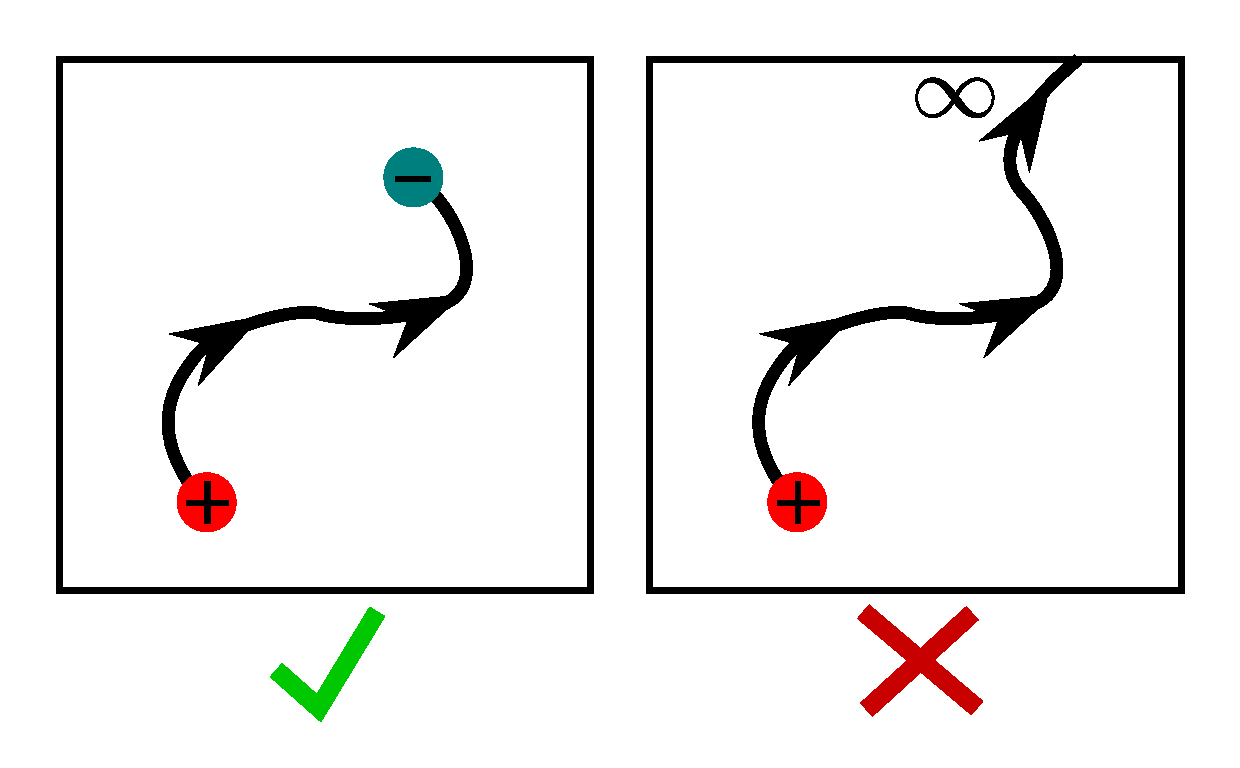
\includegraphics[width = 0.5\textwidth]{Multi-structures/Multipaths/no_infinite_paths}
}
\end{tabular}
\end{center}




\section{Multi-surfaces}

An oriented surface is a surface that has a ``front" side and a ``back" side. The orientation is depicted as arrows that point outwards from the front side, as depicted in the examples below.

\begin{center}
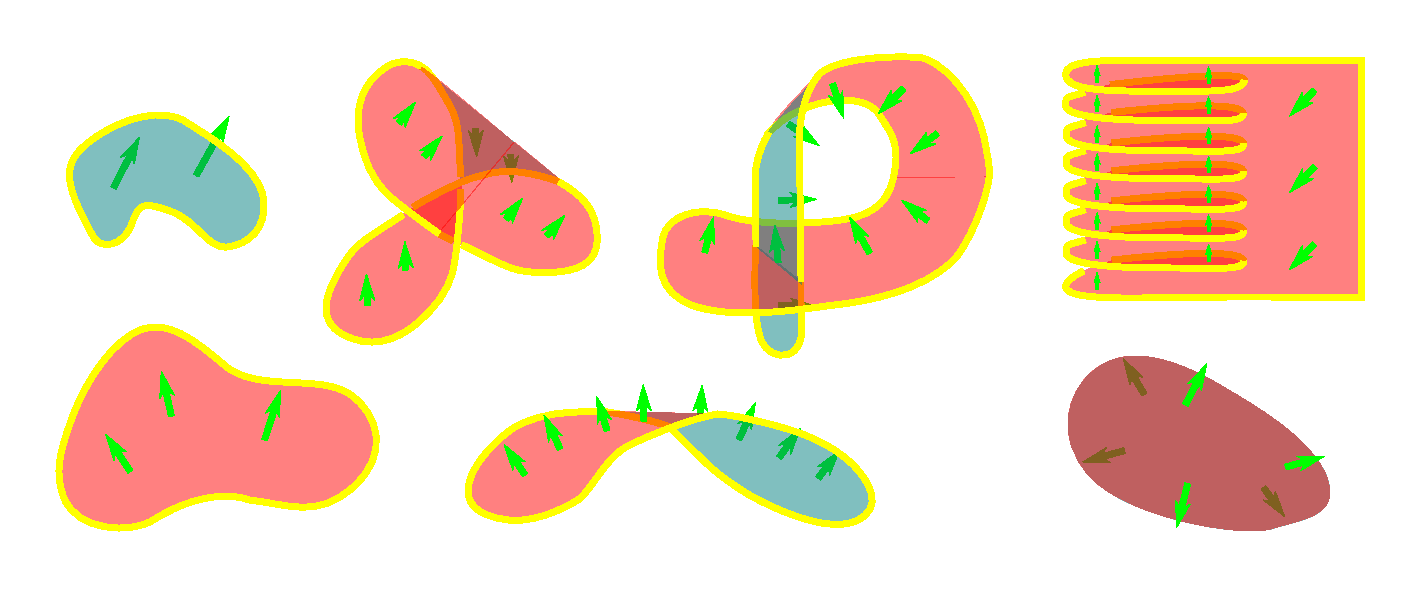
\includegraphics[scale = 0.7]{Multi-structures/Multisurfaces/oriented_surfaces}
\end{center}

A ``Mobius strip" (left) or a ``Klein bottle" (right) are examples of surfaces that have only one side, and therefore cannot be oriented without the introduction of a seam. 

\begin{tabular}{cc}
\parbox{0.5\textwidth}{
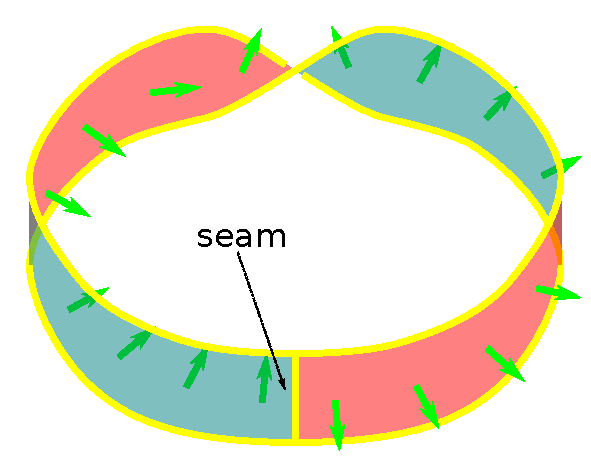
\includegraphics[scale = 0.7]{Multi-structures/Multisurfaces/Mobius_strip}
} & \parbox{0.5\textwidth}{
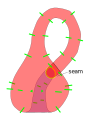
\includegraphics[scale = 0.5]{Multi-structures/Multisurfaces/Klein_bottle}
}
\end{tabular}

\begin{tabular}{cc}
\parbox{0.5\textwidth}{
A \textbf{multi-surface} is a superposition of oriented surfaces. One such superposition is depicted on the right.
} & \parbox{0.5\textwidth}{
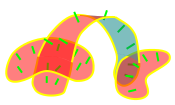
\includegraphics[width = 0.5\textwidth]{Multi-structures/Multisurfaces/multi-surface_simple}
}
\end{tabular}

\begin{tabular}{cc}
\parbox{0.5\textwidth}{
When two oriented surfaces in the same multi-surface are equivalent, the result is the common oriented surface with a weight of \(2\). When three oriented surfaces in the same multi-surface are the equivalent, the result is the common oriented surface with a weight of \(3\). Every oriented surface in a multi-surface has associated with it a ``weight" which is the number of ``stacked" oriented surfaces. The weight can be a fraction, so there can be fractional copies of a surface. {\bf If the weight is negative, then the orientation of the surface is reversed and the sign is flipped to positive.} On the right is a multi-surface where the surfaces have different weights. Note how there are no negative weights, as a negative weight merely flips the orientation of the surface.  
} & \parbox{0.5\textwidth}{
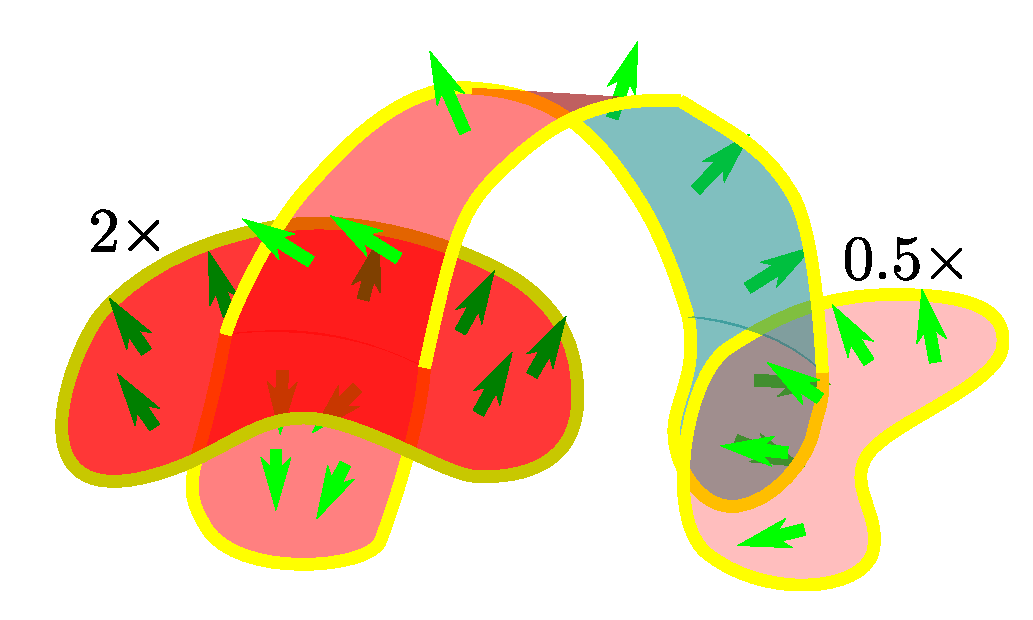
\includegraphics[width = 0.5\textwidth]{Multi-structures/Multisurfaces/multi-surface_multiplicity}
}
\end{tabular}

\vspace{2mm}

A multi-surface \(\mathbf{F}\) is effectively a set of oriented surface (\(\sigma\)) / weight (\(w\)) pairs:
\[\mathbf{F} = w_1 \sigma_1 + w_2 \sigma_2 + ... + w_N \sigma_N\]
where \(w_i\) is the weight that is assigned to surface \(\sigma_i\). This notation effectively denotes that a multi-surface is a collection/sum of oriented surfaces.

As with multi-paths, each weight \(w_i\) will be assumed to be strictly positive, as an oriented surface with a weight of 0 is not included as part of the multi-surface, and a negative weight can be made positive while reversing the surface's orientation. Moreover, the oriented surfaces will be assumed to all be unique. If a surface appears multiple times, then these appearances can be condensed into a single appearance whose weight is the sum of all weights from the multiple appearances. If an oriented surface and its reversed orientation appears, then these instances cancel out. The orientation with the smaller weight is eliminated, while the orientation with the larger weight has its weight reduced by the smaller weight. If the weights of both orientations are equal, then the orientations completely cancel each other out. It should also be noted that surfaces can partially cancel each other out (as illustrated below on the right). 

Two multi-surfaces are equivalent if and only if the networks of oriented surfaces are equivalent, regardless of how the network is broken up into individual oriented surfaces, as illustrated below. In the example on the right, the segments that are on top of each other and have opposite orientations have canceled each other out.     
\begin{center}
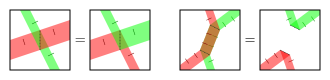
\includegraphics[scale = 0.5]{Multi-structures/Multisurfaces/multi-surface_decomposition}
\end{center}

\begin{center}
\begin{tabular}{cc}
\parbox{0.5\textwidth}{
Unless otherwise specified, no surface will be allowed to diverge to points that are infinitely distant.
} & \parbox{0.5\textwidth}{
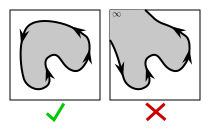
\includegraphics[width = 0.5\textwidth]{Multi-structures/Multisurfaces/no_infinite_surfaces}
}
\end{tabular}
\end{center}





\section{Multi-volumes}

~

\begin{tabular}{cc}
\parbox{0.5\textwidth}{
A \textbf{multi-volume} is a superposition of volumes. One such superposition is depicted on the right.
} & \parbox{0.5\textwidth}{
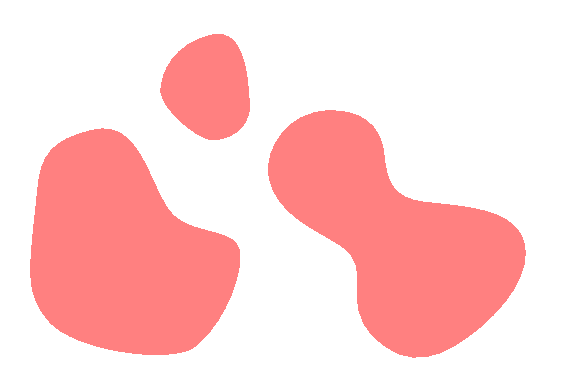
\includegraphics[scale = 0.75]{Multi-structures/Multivolumes/multi-volume_simple}
}
\end{tabular}

\begin{tabular}{cc}
\parbox{0.5\textwidth}{
When two volumes in the same multi-volume are equivalent, the result is the common volume with a weight of \(2\). When three volumes in the same multi-volume are equivalent, the result is the common volume with a weight of \(3\). Every volume in a multi-volume has associated with it a ``weight" which is the number of ``stacked" volumes. The weight can be a fraction, so there can be fractional copies of a volume. The weight can also be negative, so there can be ``anti-volume". If the weight is \(0\), then the volume is simply not included. On the right is a multi-volume, where the volumes have different weights.
} & \parbox{0.5\textwidth}{
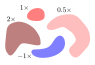
\includegraphics[scale = 0.75]{Multi-structures/Multivolumes/multi-volume_multiplicity}
}
\end{tabular}

\vspace{2mm}

A multi-volume \(U\) is effectively a set of volume (\(\Omega\)) /weight (\(w\)) pairs:
\[U = w_1 \Omega_1 + w_2 \Omega_2 + ... + w_N \Omega_N\]
where \(w_i\) is the weight that is assigned to volume \(\Omega_i\). This notation effectively denotes that a multi-volume is a collection/sum of volumes.

Each weight \(w_i\) will be assumed to be nonzero, as a volume with a weight of 0 is not included as part of the multi-volume. Moreover, the volumes will be assumed to all be unique. If a volume appears multiple times, then these appearances can be condensed into a single appearance whose weight is the sum of all weights from the multiple appearances. It should also be noted that volumes can partially cancel each other out.  

Two multi-volumes \(U_1\) and \(U_2\) are equivalent if and only if at every position \(\mathbf{q}\), the net number of volumes from \(U_1\) that contain \(\mathbf{q}\) is equal to the net number of volumes from \(U_2\) that contain \(\mathbf{q}\). Negative volumes subtract from the number of volumes that contain \(\mathbf{q}\). This is illustrated below. 

Consider the first example on the left. Left of the \(=\) sign, there is a volume with a weight of \(+1\), and a volume with a weight of \(-1\) that overlap. Right of the \(=\) sign, the volume with a weight of \(+1\) has been broken into two separate volumes, and the overlap has been canceled out. {\bf These two multi-volumes are equivalent.} 

Consider the second example on the right. Left of the \(=\) sign, there is a volume with a weight of \(+1\), and a volume with a weight of \(-1\) that overlap each other. Right of the \(=\) sign, the intersection has been canceled out, breaking each of the volumes into 2 separate pieces. {\bf These two multi-volumes are equivalent.}  

\begin{center}
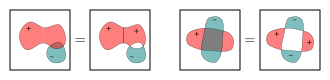
\includegraphics[scale = 0.5]{Multi-structures/Multivolumes/multi-volume_decomposition}
\end{center}

In general, given an arbitrary position \(\mathbf{q}\), and a multi-volume \(U\), the notation \(U(\mathbf{q})\) will denote the net number of volumes that contain \(\mathbf{q}\). Multi-volumes \(U_1\) and \(U_2\) are equivalent if and only if \(U_1(\mathbf{q}) = U_2(\mathbf{q})\) at all positions \(\mathbf{q}\). 

\begin{center}
\begin{tabular}{cc}
\parbox{0.5\textwidth}{
Unless otherwise specified, no volume will be allowed to diverge to points that are infinitely distant.
} & \parbox{0.5\textwidth}{
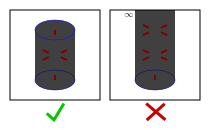
\includegraphics[width = 0.5\textwidth]{Multi-structures/Multivolumes/no_infinite_volumes}
}
\end{tabular}
\end{center}



\section{Summary}

This chapter gave an introduction to the 4 types of multi-structures that will be used in the beginning chapters of this book: multi-points; multi-paths; multi-surfaces; and multi-volumes. In the later chapters when time is introduced as a factor, an additional multi-structure called ``multi-events" will be introduced.


